\section{Leakage Assessment}
\begin{frame}{\VideoName}
    \tableofcontents[currentsection]
\end{frame}

\begin{frame}{Motivation}
    \begin{itemize}
        \item In the next section, we will see various SCA attacks on cryptographic implementations.
        \item As a developer, one might want to evaluate the DUT and conclude if it is vulnerable against SCA or not.
        \item Different new attacks are being developed and it is impractical to verify the security of our device against all of them.
        \item Leakage assessment aims to solve this problem by analyzing the power trace and answering the question of whether any input-dependent information can be detected in the traces of the DUT.
        \item We will see a method based on the \textit{student's $t-$test}.
        \item The methodology is also referred to as \textit{test vector leakage assessment (TVLA)}.
    \end{itemize}
\end{frame}

\begin{frame}{Remark}
    \begin{itemize}
        \item Leakage assessment methods do not provide any conclusions in cases where data-dependent leakage is not detected. 
        \item The absence of data-dependent leakage indicated by a particular method does not prove that the implementation is leakage-free.
    \end{itemize}
\end{frame}

\begin{frame}{Recall -- Leakages}
    \begin{itemize}
        \item We refer to the power consumption as the \textit{leakage} of the device.
       \item We consider the leakage consisting of two parts: \textit{signal} and \textit{noise}.
       \item Signal refers to the part of the leakage that contains useful information for our attack and the rest is noise.
       \begin{itemize}
           \item For example, if we would like to recover the hamming weight of an intermediate value, then the part of the leakage correlated to the hamming weight of that intermediate value is our signal.
       \end{itemize}
    \end{itemize}
\end{frame}

\begin{frame}{TVLA Step 1}
\textbf{Identify the cryptographic implementation for analysis}
    \begin{itemize}
        \item In principle, TVLA can be used for analyzing leakages of implementations for any type of algorithm.
    In practice, they are mostly used for the analysis of symmetric block cipher implementations.
    \end{itemize}
\begin{example}
    We will analyze the security of our PRESENT implementation against SCA
\end{example}
\end{frame}

\begin{frame}{TVLA Step 2}
    \textbf{Choose the intermediate value $\boldsymbol{v}$ to analyze}.
    \begin{itemize}
        \item  TVLA tests if different values of $\boldsymbol{v}$ result in different signals.
        \item The choice of $\boldsymbol{v}$ determines how we measure our traces.
    \end{itemize}
    \begin{example}
        For the attacks that we will see in next section, we will focus on the $0$th Sbox output in the first round of PRESENT.
        For this reason, here we choose this Sbox output to be our $\boldsymbol{v}$.
    \end{example}
\end{frame}

\begin{frame}{TVLA Step 3}
    \textbf{Experimental setup and measure leakages}.
    \begin{itemize}
        \item As we can imagine, for the actual attacks, experimental setups are crucial factors for success.
        \item For leakage assessment, it would be better to carry out measurements with equipment that is expected to be used by attackers that we would like to protect against.
        \item Choose two different fixed values of $\boldsymbol{v}$
        \item Measure two datasets, $\mathcal{T}_1$ and $\mathcal{T}_2$, one for each fixed value of $\boldsymbol{v}$
    \end{itemize}
    \begin{example}
    \begin{itemize}
        \item We will choose values \texttt{0} and \texttt{F} of the Sbox output to analyze.
        \item Recall \datarantwo: This dataset contains 10000 traces with a random round key and a random plaintext for each trace.
        \item $\mathcal{T}_1$ is given by subset of \datarantwo that correspond to $\boldsymbol{v}=\texttt{0}$
        \item $\mathcal{T}_2$ is given by subset of \datarantwo that correspond to $\boldsymbol{v}=\texttt{F}$
    \end{itemize}
    \end{example}
\end{frame}

\begin{frame}{TVLA Step 4a}
    \textbf{Compute sample means for leakages at one time sample.}
    \begin{itemize}
        \item Fix a time sample, let $\ell_1$ and $\ell_2$ be the leakages at this time sample from $\mathcal{T}_1$ and $\mathcal{T}_2$ respectively
        \item Compute sample means, i.e. averages, denoted $\overline{\ell}_1$ and $\overline{\ell}_2$, for $\ell_1$ and $\ell_2$
    \end{itemize}
    \begin{example}
        Let us focus on the time sample $392$.
        The sample means $\overline{\ell}_1$ and $\overline{\ell}_2$ for $\ell_1$ and $\ell_2$ are given by
        \[
        \overline{\ell}_1 = -0.04246,\quad \overline{\ell}_2=-0.05391
        \]
    \end{example}
\end{frame}

\begin{frame}{TVLA Step 4b}
    \textbf{Compute sample variances for leakages at one time sample.}
    \begin{itemize}
        \item For the same fixed time sample
        \item Let $M_1$ and $M_2$ denote the cardinalities of $\ell_1$ and $\ell_2$ respectively 
        \item Compute sample variances $s_1^2$ and $s_2^2$ for $\ell_1$ and $\ell_2$
        \begin{itemize}
            \item The sample variance $s_1^2$ of $\ell_1$ is computed by multiplying the variance of $\ell_1$ by $M_1/(M_1-1)$
            \item The sample variance $s_2^2$ of $\ell_2$ is computed by multiplying the variance of $\ell_2$ by $M_2/(M_2-1)$
        \end{itemize}
    \end{itemize}
    \begin{example}
        Let us focus on the time sample $392$.
        In our case,
        \[
        M_1=634,\quad M_2=651.
        \]
        The sample variances $s_1^2$ and $s_2^2$ for $\ell_1$ and $\ell_2$ are given by
        \[
        \overline{\ell}_1 = 2.2962\times10^{-6},\quad \overline{\ell}_2=2.7378\times10^{-6}
        \]
    \end{example}
\end{frame}

\begin{frame}{TVLA Step 4c}
    \textbf{$t-$test for one time sample}
    \begin{itemize}
        \item Now we are ready to carry out the $t-$test for our fixed time sample
        \item We first compute
        \[
        s_p^2=\frac{(M_1-1)s_1^{2}+(M_2-1)s_2^{2}}{M_1+M_2-2}
        \]
        \item Then the $t-$value is given by
        \[
        t-\text{value}:=\frac{\overline{\ell}_1-\overline{\ell}_2}{\sqrt{s_p^2(1/M_1+1/M_2)}}.
        \]
        \item TVLA has a threshold $4.5$, in case the absolute value $|t|-$value $>4.5$, we consider the leakages at this time sample to be potentially exploitable
        \item This choice is based on statistical hypothesis testing techniques
    \end{itemize}
    \begin{example}
    \begin{itemize}
        \item The $t-$value at time sample $392$ is given by $129.27$, which is much higher than the threshold.
    \end{itemize}
    \end{example}
\end{frame}

\begin{frame}{All traces and $50$ traces, dotted line correspond to threshold}
    \begin{figure}[h]
    \centering
    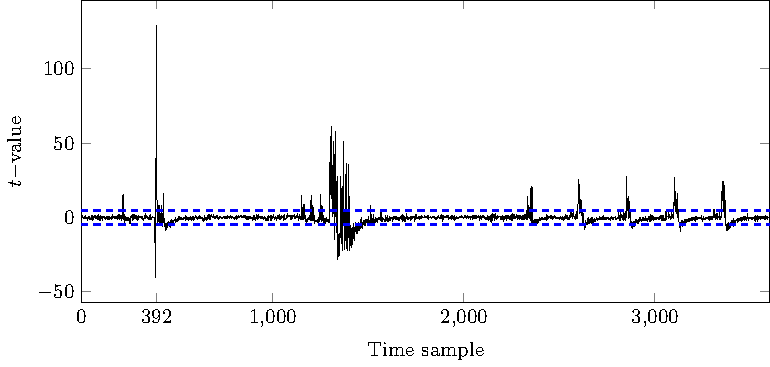
\includegraphics[width=0.55\textwidth]{fig/TVLA_sbox.pdf}
\end{figure}
    \begin{figure}[h]
    \centering
    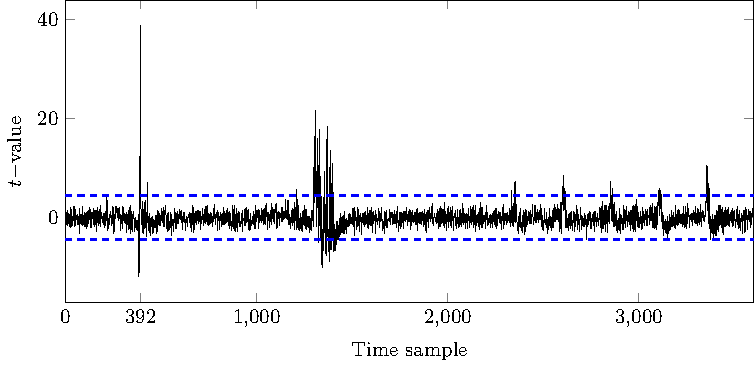
\includegraphics[width=0.55\textwidth]{fig/TVLA_sbox_less_traces.pdf}
\end{figure}
\end{frame}

\begin{frame}{Observations}
    \begin{itemize}
        \item When more traces are used, it is more likely for us to capture information about the inputs from the leakages.
        We will see in the next section that more traces indeed indicate higher chances for the attacks to be successful.
        \item The highest $|t|-$value is obtained at $392$.
        We will see that this is our \textit{point of interest} (POI) for our attack -- sample points that give the best attack results   
    \end{itemize}
    \begin{alertblock}{Remark}
        Python code for TVLA can be found here\\
        \url{https://github.com/XIAOLUHOU/SCA-measurements-and-analysis----Experimental-results-for-textbook/blob/main/Assignment_materials/TVLA.ipynb}
    \end{alertblock}
\end{frame}

\section{SNR Computations}
\begin{frame}{\VideoName}
    \tableofcontents[currentsection]
\end{frame}

\begin{frame}{Definition}
    \begin{itemize}
        \item Signal-to-noise ratio (SNR) is commonly used in electrical engineering and signal processing, the general definition is
\[
\text{SNR}=\frac{\var{\text{signal}}}{\var{\text{noise}}},
\]
\item In our case, for a fixed time sample $t$, signal, denoted $X_t$, is part of the leakage relevant to our attack.
\item Noise, denoted $N_t$, is the rest of the leakage
\item And we define
\begin{equation*}
    \text{SNR}=\frac{\var{X_t}}{\var{N_t}}.
\end{equation*}
\item $\var{X_t}$ measures how much the leakage varies at time sample $t$ due to the signal.
\item $\var{N_t}$ measures how much the leakage varies due to the noise.
\item SNR quantifies how much information is leaked at time sample $t$ from the measurements.
\item The higher the SNR, the lower the noise.
    \end{itemize}
\end{frame}

\begin{frame}{Remark}
\begin{alertblock}{Remark}
    \begin{itemize}
        \item By definition, signal is part of the leakage relevant to our attack
        \item It is thus dependent on what we are interested in during the attack
        \item Attacks with different focuses have different signal values
    \end{itemize}
\end{alertblock}
We will explain how SNR values are computed using an example
\end{frame}

\begin{frame}{SNR -- Example}
    \begin{example}
        \begin{itemize}
            \item \datarantwo: This dataset contains 10000 traces with a random round key and a random plaintext for each trace.
            \item Suppose we are interested in the exact value of the $0$th Sbox output in the first round of PRESENT. Let us denote this intermediate value by $\boldsymbol{v}$.
            \item Fix a time sample $t$
            \item Then signal $X_t$ is given by the part of the leakage related to $\boldsymbol{v}$.
            \item To compute $\var{X_t}$, we first divide the traces into $16$ sets: $A_1,A_2,\dots,A_{16}$, where $A_i$ contains traces corresponding to $\boldsymbol{v}=i-1$
            \item Take $t=600$.
            \item We compute the average of the trace leakages at $t=600$ across each set, which can be considered as approximation of the signals
            \[
0.08212,\quad0.08221,\quad0.08209,\quad\dots
\]
        \end{itemize}
    \end{example}
\end{frame}

\begin{frame}{SNR -- Example}
    \begin{example}
        \begin{itemize}
            \item Take $t=600$.
            \item We compute the average of the trace leakages at $t=600$ across each set, which can be considered as approximation of the signals
            \[
0.08212,\quad0.08221,\quad0.08209,\quad\dots
\]
\item Then the variance of $X_t$ is given by the variance of those average values
\[
\var{X_{600}}\approx1.0088\times10^{-8}
\]
\item The noise in each trace at $t=600$ is given by the leakage minus the corresponding average, and we have
\[
\var{N_t}\approx6.4184\times10^{-6}
\]
        \end{itemize}
    \end{example}
\end{frame}

\begin{frame}{SNR -- Example}
    \begin{example}
        \begin{itemize}
            \item We are interested in the exact value of the $0$th Sbox output, denoted by $\boldsymbol{v}$.
            \item We divide the traces into $16$ sets: $A_1,A_2,\dots,A_{16}$, where $A_i$ contains traces corresponding to $\boldsymbol{v}=i-1$
            \item Take time sample $t=600$.
\[
\var{X_{600}}\approx1.0088\times10^{-8},\quad
\var{N_t}\approx6.4184\times10^{-6}
\]
\item $\text{SNR}_{600}\approx0.00157$
\item The same computations can be done for other time samples
        \end{itemize}
    \end{example}
\end{frame}

\begin{frame}{$\var{X_t}$}
\begin{figure} 
        \centering
        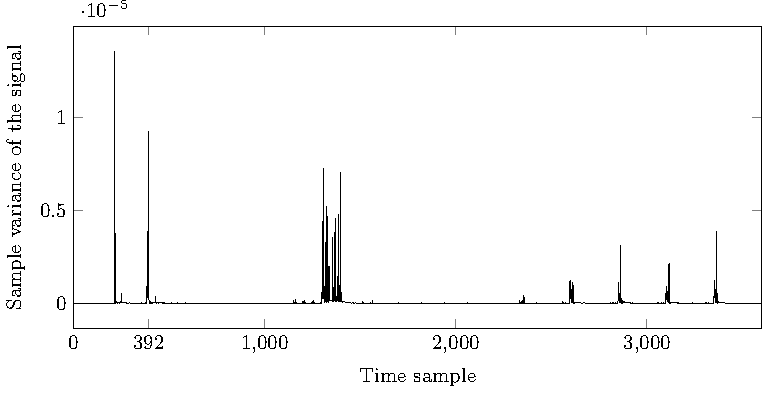
\includegraphics{fig/signal_identity_model.pdf}
        \caption{
        % Sample variance of the signal, \datarantwo.
        The signal is given by the exact value of the $0$th Sbox output.}
    \end{figure}
\end{frame}

\begin{frame}{SNR}
     \begin{figure} 
        \centering
        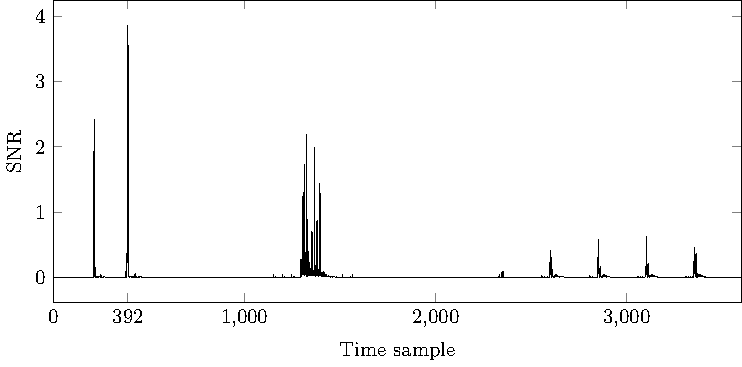
\includegraphics{fig/SNR_identity_model.pdf}
        \caption{
        The signal is given by the exact value of the $0$th Sbox output.}
    \end{figure}
\end{frame}

\begin{frame}{Comparison -- $\var{X_t}$ and SNR}
    \begin{figure}
        \centering
        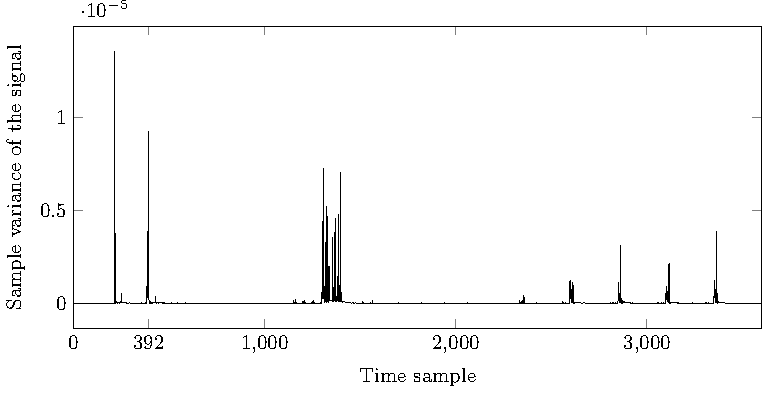
\includegraphics[width=0.5\textwidth]{fig/signal_identity_model.pdf}
    \end{figure}
    \begin{figure}
        \centering
        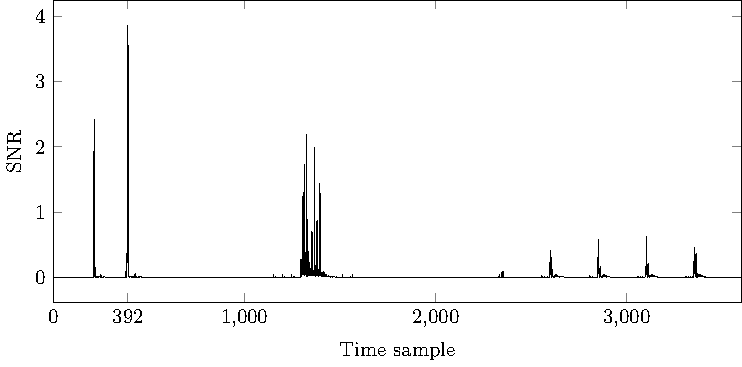
\includegraphics[width=0.5\textwidth]{fig/SNR_identity_model.pdf}
    \end{figure}
\end{frame}

\begin{frame}{Recall -- averaged trace}
    \begin{figure}
    \centering
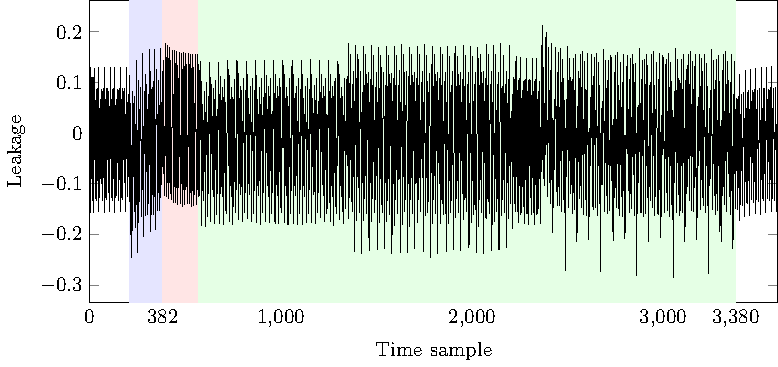
\includegraphics{fig/PRESENT_plot___one_round_average___highlighted_operations.pdf}
    \caption{The averaged trace for $5000$ traces from the \datafixone.
    The blue, pink, and green parts of the trace correspond to addRoundKey, sBoxLayer, and pLayer respectively.}
\end{figure}
\end{frame}

\begin{frame}{$\var{N_t}$}
    \begin{figure}
        \centering
        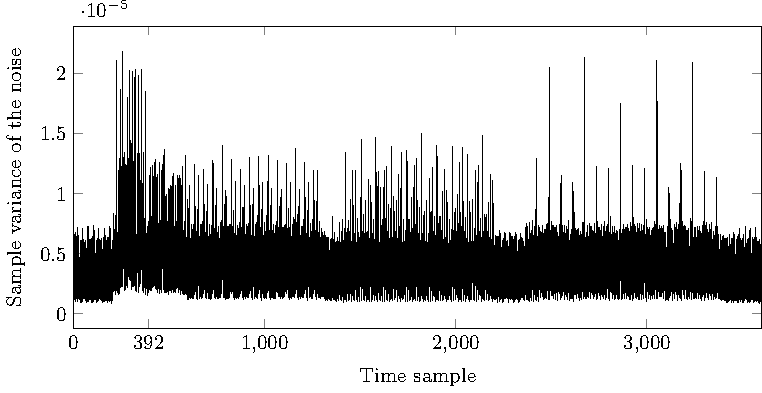
\includegraphics{fig/noise_identity_model.pdf}
        \caption{
        The signal is given by the exact value of the $0$th Sbox output.}
    \end{figure}
\end{frame}

\begin{frame}{Noise and averaged trace}
 \begin{figure}
        \centering
        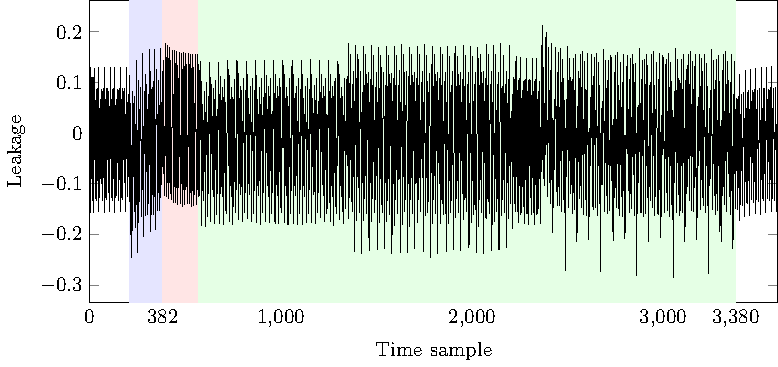
\includegraphics[width=0.5\textwidth]{fig/PRESENT_plot___one_round_average___highlighted_operations.pdf}
    \end{figure}
    \begin{figure}
        \centering
        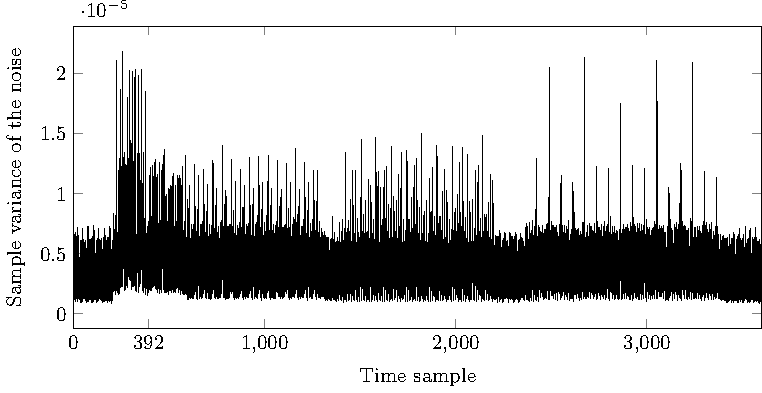
\includegraphics[width=0.5\textwidth]{fig/noise_identity_model.pdf}
    \end{figure}
\end{frame}

\begin{frame}{Observations}
    \begin{itemize}
        \item The shape of variance of noise has similarities to one round of PRESENT computations -- most of the leakage is not related to $\boldsymbol{v}$. 
        \item The peaks for the variance of signal and SNR correspond to each other.
        \item The first two peaks are likely related to AddRoundKey and sBoxLayer.
        \item We can deduce that the peak at $t=392$ is related to the $0$th Sbox computation
       \item The peaks after $1000$ are probably caused by the permutation of the $4$ bits of $\boldsymbol{v}$, the $0$th Sbox output.
    \end{itemize}
\begin{alertblock}{Remark}
    The code for the computation with $\boldsymbol{v}$ can be found here:
    \begin{center}
    \url{https://github.com/XIAOLUHOU/SCA-measurements-and-analysis----Experimental-results-for-textbook/blob/main/Assignment_materials/SNR_Computation.ipynb}
    \end{center}
\end{alertblock}
\end{frame}

\begin{frame}{What if we are interested in the Hamming weight of the Sbox output}
    \begin{figure} 
        \centering
        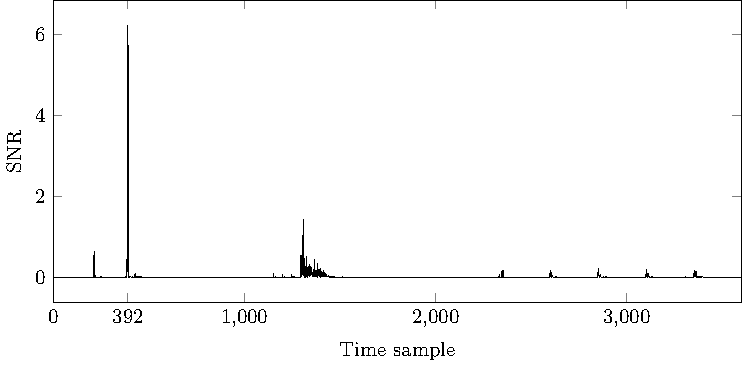
\includegraphics{fig/SNR_hw.pdf}
        \caption{
        The signal is given by the Hamming weight of the $0$th Sbox output.}
    \end{figure}
\end{frame}

\begin{frame}{Observations}
    \begin{itemize}
        \item The sample variances of the noise are very similar and resemble the leakage of PRESENT computation
        \item The peaks in the variance of signal and SNR also correspond to each other.
        \item The locations of the peaks for SNR are similar.
        \item The highest peak in both SNR figures are at time sample $392$.
\begin{itemize}
    \item This time sample corresponds to the computation of the $0$th Sbox in sBoxLayer.
    \item Higher SNR value at this point when we consider Hamming weight -- the Hamming weight leakage model is closer to the device leakage than the identity leakage model
\end{itemize}
    \end{itemize}
\end{frame}

\begin{frame}{POIs}
    \begin{itemize}
        \item Normally in DPA attacks, we would like to focus on time samples where the corresponding SNRs are high.
        \item We refer to those time samples as \textit{points of interest (POIs)}.
        \item Signal given by exact value of $\boldsymbol{v}$
        \begin{itemize}
             \item One POI $t=392$.
             \item Three POIs: $t=392,218,1328$
        \end{itemize}
        \item Signal given by the Hamming weight of $\boldsymbol{v}$
        \begin{itemize}
             \item One POI $t=392$.
             \item Three POIs: $t=392,1309,1304$
        \end{itemize}
    \end{itemize}
\end{frame}

\section{Final Remarks}
\begin{frame}{\VideoName}
    \tableofcontents[currentsection]
\end{frame}

\begin{frame}{Leakage assessment and SNR}
    \begin{itemize}
        \item Leakage assessment is often used in the early stages of evaluating a cryptographic implementation’s security to determine whether it leaks information through side channels.
        \item SNR is used to find the POIs for an attack
    \end{itemize}

    \begin{itemize}
        \item Leakage assessment determines whether side-channel leakage is statistically significant and detectable
        \item SNR quantifies how much of the side-channel signal is useful relative to noise.
    \end{itemize}
\end{frame}

\begin{frame}{Section summary}
    \begin{itemize}
        \item Power consumption side-channel leakages come from the switching power in CMOS-based circuits
        \item Power analysis attacks utilize an oscilloscope for capturing the traces
        \item The captured power consumption, or so-called leakage, is dependent on both operation and data in the DUT
        \item Leakage assessment can be used to assess the cryptographic implementation’s security to determine if it leaks information through side channels.
        \item SNR computations can help to identify the point of interest for our attack
    \end{itemize}
\end{frame}